\documentclass[english,,man]{apa6}
\usepackage{lmodern}
\usepackage{amssymb,amsmath}
\usepackage{ifxetex,ifluatex}
\usepackage{fixltx2e} % provides \textsubscript
\ifnum 0\ifxetex 1\fi\ifluatex 1\fi=0 % if pdftex
  \usepackage[T1]{fontenc}
  \usepackage[utf8]{inputenc}
\else % if luatex or xelatex
  \ifxetex
    \usepackage{mathspec}
  \else
    \usepackage{fontspec}
  \fi
  \defaultfontfeatures{Ligatures=TeX,Scale=MatchLowercase}
\fi
% use upquote if available, for straight quotes in verbatim environments
\IfFileExists{upquote.sty}{\usepackage{upquote}}{}
% use microtype if available
\IfFileExists{microtype.sty}{%
\usepackage{microtype}
\UseMicrotypeSet[protrusion]{basicmath} % disable protrusion for tt fonts
}{}
\usepackage{hyperref}
\hypersetup{unicode=true,
            pdftitle={Inferences With Longitudinal Data},
            pdfauthor={\ldots{}},
            pdfkeywords={\ldots{}.},
            pdfborder={0 0 0},
            breaklinks=true}
\urlstyle{same}  % don't use monospace font for urls
\ifnum 0\ifxetex 1\fi\ifluatex 1\fi=0 % if pdftex
  \usepackage[shorthands=off,main=english]{babel}
\else
  \usepackage{polyglossia}
  \setmainlanguage[]{english}
\fi
\usepackage{color}
\usepackage{fancyvrb}
\newcommand{\VerbBar}{|}
\newcommand{\VERB}{\Verb[commandchars=\\\{\}]}
\DefineVerbatimEnvironment{Highlighting}{Verbatim}{commandchars=\\\{\}}
% Add ',fontsize=\small' for more characters per line
\usepackage{framed}
\definecolor{shadecolor}{RGB}{248,248,248}
\newenvironment{Shaded}{\begin{snugshade}}{\end{snugshade}}
\newcommand{\AlertTok}[1]{\textcolor[rgb]{0.94,0.16,0.16}{#1}}
\newcommand{\AnnotationTok}[1]{\textcolor[rgb]{0.56,0.35,0.01}{\textbf{\textit{#1}}}}
\newcommand{\AttributeTok}[1]{\textcolor[rgb]{0.77,0.63,0.00}{#1}}
\newcommand{\BaseNTok}[1]{\textcolor[rgb]{0.00,0.00,0.81}{#1}}
\newcommand{\BuiltInTok}[1]{#1}
\newcommand{\CharTok}[1]{\textcolor[rgb]{0.31,0.60,0.02}{#1}}
\newcommand{\CommentTok}[1]{\textcolor[rgb]{0.56,0.35,0.01}{\textit{#1}}}
\newcommand{\CommentVarTok}[1]{\textcolor[rgb]{0.56,0.35,0.01}{\textbf{\textit{#1}}}}
\newcommand{\ConstantTok}[1]{\textcolor[rgb]{0.00,0.00,0.00}{#1}}
\newcommand{\ControlFlowTok}[1]{\textcolor[rgb]{0.13,0.29,0.53}{\textbf{#1}}}
\newcommand{\DataTypeTok}[1]{\textcolor[rgb]{0.13,0.29,0.53}{#1}}
\newcommand{\DecValTok}[1]{\textcolor[rgb]{0.00,0.00,0.81}{#1}}
\newcommand{\DocumentationTok}[1]{\textcolor[rgb]{0.56,0.35,0.01}{\textbf{\textit{#1}}}}
\newcommand{\ErrorTok}[1]{\textcolor[rgb]{0.64,0.00,0.00}{\textbf{#1}}}
\newcommand{\ExtensionTok}[1]{#1}
\newcommand{\FloatTok}[1]{\textcolor[rgb]{0.00,0.00,0.81}{#1}}
\newcommand{\FunctionTok}[1]{\textcolor[rgb]{0.00,0.00,0.00}{#1}}
\newcommand{\ImportTok}[1]{#1}
\newcommand{\InformationTok}[1]{\textcolor[rgb]{0.56,0.35,0.01}{\textbf{\textit{#1}}}}
\newcommand{\KeywordTok}[1]{\textcolor[rgb]{0.13,0.29,0.53}{\textbf{#1}}}
\newcommand{\NormalTok}[1]{#1}
\newcommand{\OperatorTok}[1]{\textcolor[rgb]{0.81,0.36,0.00}{\textbf{#1}}}
\newcommand{\OtherTok}[1]{\textcolor[rgb]{0.56,0.35,0.01}{#1}}
\newcommand{\PreprocessorTok}[1]{\textcolor[rgb]{0.56,0.35,0.01}{\textit{#1}}}
\newcommand{\RegionMarkerTok}[1]{#1}
\newcommand{\SpecialCharTok}[1]{\textcolor[rgb]{0.00,0.00,0.00}{#1}}
\newcommand{\SpecialStringTok}[1]{\textcolor[rgb]{0.31,0.60,0.02}{#1}}
\newcommand{\StringTok}[1]{\textcolor[rgb]{0.31,0.60,0.02}{#1}}
\newcommand{\VariableTok}[1]{\textcolor[rgb]{0.00,0.00,0.00}{#1}}
\newcommand{\VerbatimStringTok}[1]{\textcolor[rgb]{0.31,0.60,0.02}{#1}}
\newcommand{\WarningTok}[1]{\textcolor[rgb]{0.56,0.35,0.01}{\textbf{\textit{#1}}}}
\usepackage{graphicx,grffile}
\makeatletter
\def\maxwidth{\ifdim\Gin@nat@width>\linewidth\linewidth\else\Gin@nat@width\fi}
\def\maxheight{\ifdim\Gin@nat@height>\textheight\textheight\else\Gin@nat@height\fi}
\makeatother
% Scale images if necessary, so that they will not overflow the page
% margins by default, and it is still possible to overwrite the defaults
% using explicit options in \includegraphics[width, height, ...]{}
\setkeys{Gin}{width=\maxwidth,height=\maxheight,keepaspectratio}
\IfFileExists{parskip.sty}{%
\usepackage{parskip}
}{% else
\setlength{\parindent}{0pt}
\setlength{\parskip}{6pt plus 2pt minus 1pt}
}
\setlength{\emergencystretch}{3em}  % prevent overfull lines
\providecommand{\tightlist}{%
  \setlength{\itemsep}{0pt}\setlength{\parskip}{0pt}}
\setcounter{secnumdepth}{0}
% Redefines (sub)paragraphs to behave more like sections
\ifx\paragraph\undefined\else
\let\oldparagraph\paragraph
\renewcommand{\paragraph}[1]{\oldparagraph{#1}\mbox{}}
\fi
\ifx\subparagraph\undefined\else
\let\oldsubparagraph\subparagraph
\renewcommand{\subparagraph}[1]{\oldsubparagraph{#1}\mbox{}}
\fi

%%% Use protect on footnotes to avoid problems with footnotes in titles
\let\rmarkdownfootnote\footnote%
\def\footnote{\protect\rmarkdownfootnote}


  \title{Inferences With Longitudinal Data}
    \author{\ldots{}\textsuperscript{1}}
    \date{}
  
\shorttitle{LONGITUDINAL INFERENCES}
\affiliation{
\vspace{0.5cm}
\textsuperscript{1} ...}
\keywords{....\newline\indent Word count: 95}
\usepackage{csquotes}
\usepackage{upgreek}
\captionsetup{font=singlespacing,justification=justified}

\usepackage{longtable}
\usepackage{lscape}
\usepackage{multirow}
\usepackage{tabularx}
\usepackage[flushleft]{threeparttable}
\usepackage{threeparttablex}

\newenvironment{lltable}{\begin{landscape}\begin{center}\begin{ThreePartTable}}{\end{ThreePartTable}\end{center}\end{landscape}}

\makeatletter
\newcommand\LastLTentrywidth{1em}
\newlength\longtablewidth
\setlength{\longtablewidth}{1in}
\newcommand{\getlongtablewidth}{\begingroup \ifcsname LT@\roman{LT@tables}\endcsname \global\longtablewidth=0pt \renewcommand{\LT@entry}[2]{\global\advance\longtablewidth by ##2\relax\gdef\LastLTentrywidth{##2}}\@nameuse{LT@\roman{LT@tables}} \fi \endgroup}


\DeclareDelayedFloatFlavor{ThreePartTable}{table}
\DeclareDelayedFloatFlavor{lltable}{table}
\DeclareDelayedFloatFlavor*{longtable}{table}
\makeatletter
\renewcommand{\efloat@iwrite}[1]{\immediate\expandafter\protected@write\csname efloat@post#1\endcsname{}}
\makeatother
\usepackage{lineno}

\linenumbers

\authornote{\ldots{}.

Correspondence concerning this article should be addressed to \ldots{},
\ldots{}. E-mail: \ldots{}}

\abstract{
Begin here\ldots{}


}

\usepackage{amsthm}
\newtheorem{theorem}{Theorem}[section]
\newtheorem{lemma}{Lemma}[section]
\theoremstyle{definition}
\newtheorem{definition}{Definition}[section]
\newtheorem{corollary}{Corollary}[section]
\newtheorem{proposition}{Proposition}[section]
\theoremstyle{definition}
\newtheorem{example}{Example}[section]
\theoremstyle{definition}
\newtheorem{exercise}{Exercise}[section]
\theoremstyle{remark}
\newtheorem*{remark}{Remark}
\newtheorem*{solution}{Solution}
\begin{document}
\maketitle

Organizational phenomena unfold over time. They are processes that
develop, change, and evolve (Pitariu \& Ployhart, 2010) that create a
sequence of events within a person's stream of experience (Beal, 2015).
Moreover, organizations are systems with many connected parts, and
systems are inherently dynamic. Studying these systems and processes,
therefore, requires paying attention not to static snapshots of behavior
(Ilgen \& Hulin, 2000), but variables and relationships as they move
through time; doing so puts us in a better position to capture the
sequence, understand it, and can lead to new and interesting insights
(Kozlowski \& Bell, 2003).

This sentiment is reflected in our empirical literature, where repeated
assessments are now common. For instance, Jones et al. (2016) observed
the work attitudes of pregnant women in their second trimester every
week until they gave birth. Meier and Spector (2013) examined
counterproductive work behavior over five waves. Hardy, Day, and Steele
(2018) investigated self-regulation over 20 lab trials. Finally,
Johnson, Lanaj, and Barnes (2014) observed justice behavior and resource
depletion across 10 consecutive workdays.

Armed with repeated observations, there are then different research
questions that we can explore. Jones et al. (2016) ask about trend: they
want to determine if the trajectories among certain variables increase
or decrease over time. Johnson et al. (2014) about change: they are
interested in how changes in one variable relate to changes in another
across time. Hardy et al. (2018) inquire about dynamic relationships,
where prior values on one variable predict subsequent values on another,
and this second variable then goes back to predict the first at a later
point in time. Finally, Meier and Spector (2013) examine how effect
sizes change when they vary the time lag between their independent and
dependent variable.

Researchers then evoke statistical models that are determined by their
research questions. Meier and Spector (2013) present a sequence of path
models that test increasingly longer time lags. Hardy et al. (2018) and
Jones et al. (2016) employ bivariate cross-lagged latent growth curves,
an approach similar to the latent change model used by Ritter, Matthews,
Ford, and Henderson (2016) We also find complex hierarchical linear
models in many event-sampling studies (e.g., Koopman, Lanaj, \& Scott,
2016; Rosen, Koopman, Gabriel, \& Johnson, 2016).

The spine of an investigation, finally, is to interpret the model and
make an inference regarding the original question. Jones et al. (2016)
infer negative slopes for concealing behaviors and positive slopes for
revealing behaviors. Johnson et al. (2014) state that justice behaviors
fluctuate day to day and predict changes in depletion. Hardy et al.
(2018) find support for dynamic relationships between self-efficacy,
metacognition, and exploratory behaviors. Finally, Meier and Spector
(2013) suggest that the effects of work stressors on counterproductive
work behaviors are not substantially different across different time
lags.

None of these inferences perfectly discovers the data generating
mechanism. Rather, each asks an interesting and important question about
how DVs relate to IVs. Only with lots of asking about lots of different
patterns of relationships across the variables could we piece together
one (of many) possible representation(s) of the data generating process
-- hopefully having a good theory to guide the way.

We want to link inferences to models in this paper so that researchers
know which of the many models they can use when they are interested in
one of the many possible inferences in a longitudinal investigation. As
should be clear to anyone reading our literature, there is great
excitement for the utility of longitudinal studies; they can pose
interesting questions and discover patterns that would otherwise be
impossible to capture in a static investigation. We bring attention to
the span of questions available so that researchers can fully appreciate
and take advantage of their data. Although the inferences concern
trajectories or relationships over time, their small differences have
large implications for what we take away from them -- what we ultimately
conclude. Moreoever, there are many inferences, many models, and
different models can be used to understand or explore the same
inference. In this paper, we provide readers with a specific model for
each inference so that they can be sure that the model they evoke is
appropriate for the research question that they are interested in. In
summary, this paper exposes researchers to the span of inferences they
may investigate when they collect longitudinal data, links those
inferences to models, and parses some of the modeling literature that
may be difficult to consume for researchers with only graduate level
training in statistics.

Below, we do these things.

\hypertarget{longitudinal-definitions}{%
\section{Longitudinal Definitions}\label{longitudinal-definitions}}

This paper is exclusively devoted to the inferences we make with
repeated observations, so we begin by identifying a few labels and
definitions. Authors typically identify a \enquote{longitudinal} study
by making a contrast with respect to either a) research designs or b)
data structures. Longitudinal \emph{research} is different from
cross-sectional research because longitudinal designs entail three or
more repeated observations (Ployhart \& Vandenberg, 2010). We therefore
emphasize differences on the number of observations when we distinguish
longitudinal from other types of research. Longitudinal \emph{data} are
repeated observations on several units (i.e., \(N\) or \(i\)
\textgreater{} 1), whereas panel data are observations of one unit over
time -- a distinction that focuses on the amount of people in our study
(given repeated measures). Most organizational studies collect data on
more than one unit, therefore our discussion below focuses on
longitudinal research with longitudinal data, or designs with \(N\)
\textgreater{} 1, \(t\) \textgreater{}= 3, and the same construct(s)
measured on (potentially) each \(i\) at (potentially) each \(t\).

\hypertarget{framework}{%
\subsection{Framework}\label{framework}}

Level. Trend. Dynamics. These are umbrella research foci, each has its
own sub-inferences and models. Each section will basically have two
notions: trying to understand the thing itself (one variable). Looking
at trend or variability in trend. Then looking at correlates or
predictors of the thing: correlates of trend, etc.

Each section will also point to models. But there is nuance. The models
have different names, some require stationary, some don't. You need to
appreciate that and make sure you are attending to all of its nuance.
All we are doing here is pointing you in the direction.

\hypertarget{level}{%
\section{Level}\label{level}}

Level inferences concern the value that a variable takes (high or low)
across time. If we put a variable on the y-axis and plot its values
against time on the x-axis, what value does it take at time \(t\), or
what value does it take on average, across time, or what value does it
take within certain windows of time?

Level has to do with the condition of a state with respect to its state
space. It may have a state space of zero to ten, and its current
condition is seven. This is level. It has also been called magnitude.

Is affect high, on average, across time? Is trainee skill low at the
beginning of a training session? Are newcomer perceptions of unit
climate high at the end of a two-week socialization process?

Level, with respect to a certain point or window in time, is called the
intercept in the statistical literature, and we can make an inference
about the intercept at any observation point. Sometimes we are
interested in the level at the beginning of the study, other times we
are interested in the level at the last observation. We can of course
also be interested in the average level across time.

When we retain one variable but add multiple units -- people or
organizations, for example -- then we can look at the variability in
level. Does everyone have high affect across time? Is there variability
in the level of skill among trainees at the beginning of a training
session? Now there are multiple points on our graph at each time.

When we measure two or more variables we can examine all of their
levels, but we can also correlate them, or regress some variables onto
others. Is the level of affect related to the level of helping behaviors
across time? That is, when affect is high, are helping behaviors also
high or are they low? When team cohesion is low, is team performance low
as well, or is it high?

figure \ref{level}

\hypertarget{inference-list}{%
\subsection{Inference List}\label{inference-list}}

The level of \(x\) at time \(t\) is\ldots{} Picture 1.

There is variability in the level of \(x\) at time \(t\). Picture 2.

There is a relationship between the levels of multiple variables. \(x\)
relates to \(y\) across time. Stable vs fluctuating \(x\),
time-invariant vs time-varying covariates.

\hypertarget{pictures}{%
\subsection{Pictures}\label{pictures}}

One Variable, one unit.

\begin{figure}
\centering
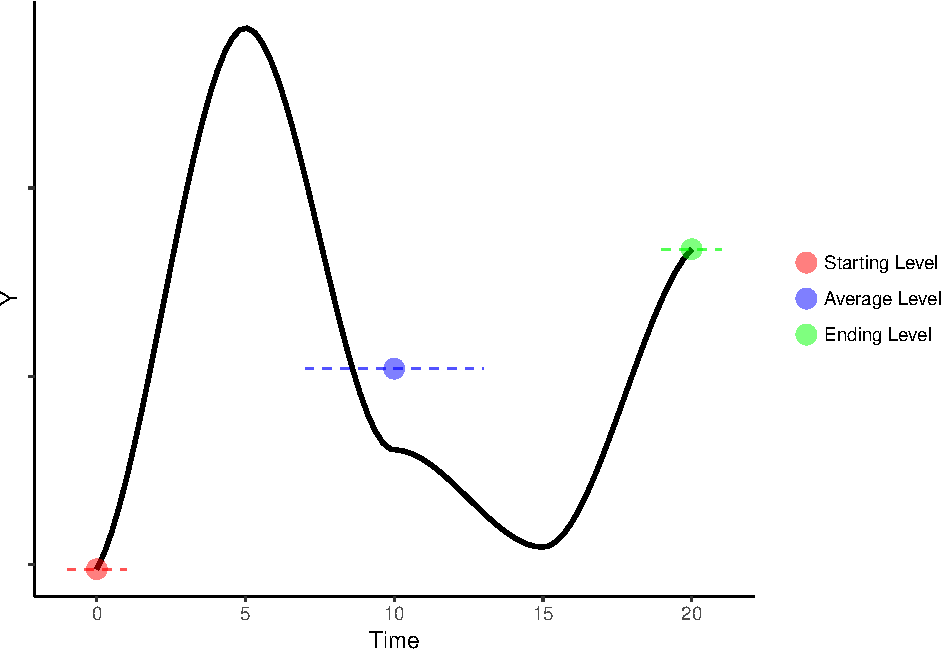
\includegraphics{figures/unnamed-chunk-7-1.pdf}
\caption{\label{fig:unnamed-chunk-7}something here\label{level}}
\end{figure}

One variable, multiple units

\begin{figure}
\centering
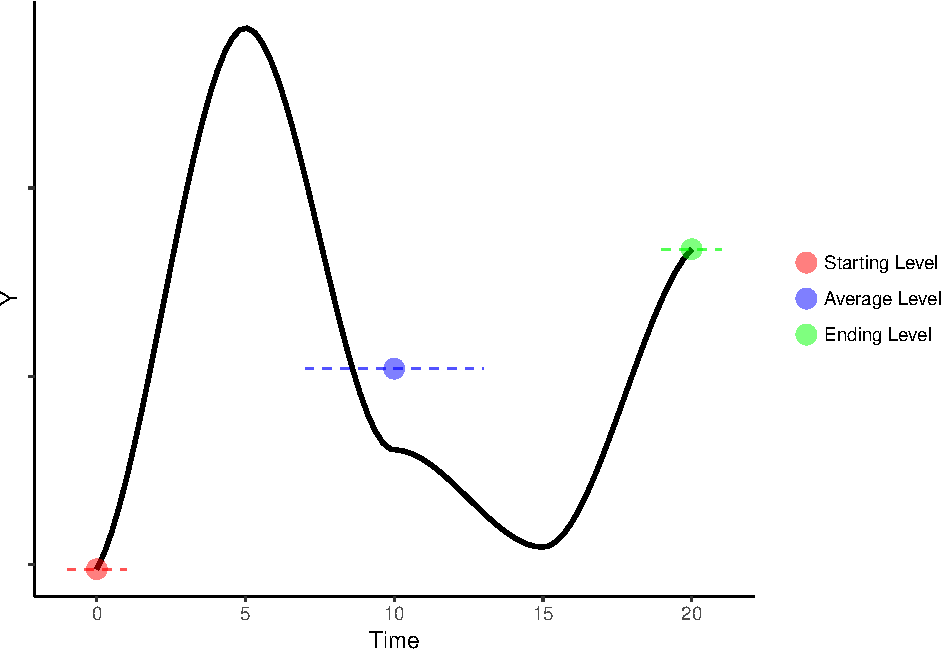
\includegraphics{figures/unnamed-chunk-8-1.pdf}
\caption{\label{fig:unnamed-chunk-8}another\label{level_var}}
\end{figure}

Muliple Variables

When affect is low performance is low. When affect is high performance
is high.

\begin{figure}
\centering
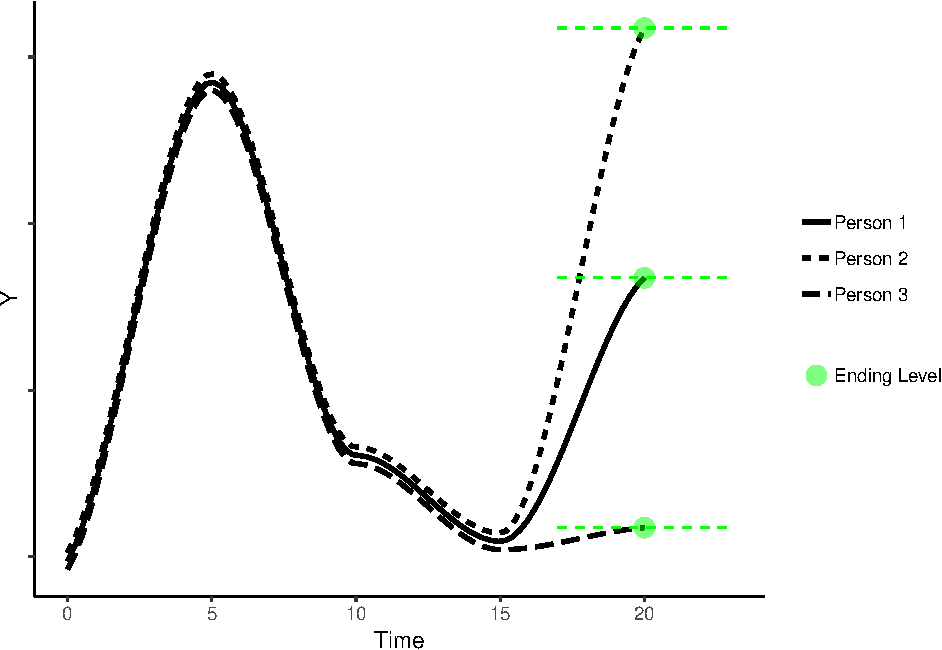
\includegraphics{figures/unnamed-chunk-9-1.pdf}
\caption{\label{fig:unnamed-chunk-9}double\label{level_relation}}
\end{figure}

\hypertarget{models}{%
\subsection{Models}\label{models}}

Intercept only models: these can be done in HLM or SEM. Time-varying or
invariant covariates analysis, these can be done in HLM or SEM. Point to
references.

\hypertarget{trend}{%
\section{Trend}\label{trend}}

Trend has to do with the global shape of the trajectory across time. If
we put a variable on the y-axis and plot its values against time on the
x-axis, do the values tend to go up or down over time? Trend can be
thought of as the coarse-grained direction of a trajectory. Also
referred to as growth.

Does affect go up or down across our measurement period, or is it
relatively stable? Does trainee skill increase over the training
session?

These are all linear examples of trend. We can also look at curvilinear
things. Do newcomer perceptions of the positive attitude in the
workplace increase and then plateua over time? Does the response time of
a medical team decrease with each successive case but then remain stable
once every crew member has reached their maximum potential to coordinate
their actions?

The statistical term for trend is slope, and linear slopes are straight
lines whereas curvilinear slopes bend across time.

When we examine more than one unit on a variable we can also look at the
variability in trend. Do all trainees develop greater skill across time?
Is there variability in the trend of helping behaviors, or
counterproductive work behaviors over time?

When we examine two or more variables, we can of course look at trend or
slope in each of them. The next step is to then correlate slopes or
regress one slope on another. Does the trend in affect relate to the
trend in helping behaviors?

\hypertarget{inference-list-1}{%
\subsection{Inference List}\label{inference-list-1}}

There is growth in a variable across time. Its slope/trend is positive
or negative.

There is variability in the growth of a variable across time.
Slopes/trends differ across units.

There are correlates/predictors of trend.

There is a relationship between two growth curves. Two trends are
correlated.

\hypertarget{pictures-1}{%
\subsection{Pictures}\label{pictures-1}}

\begin{figure}
\centering
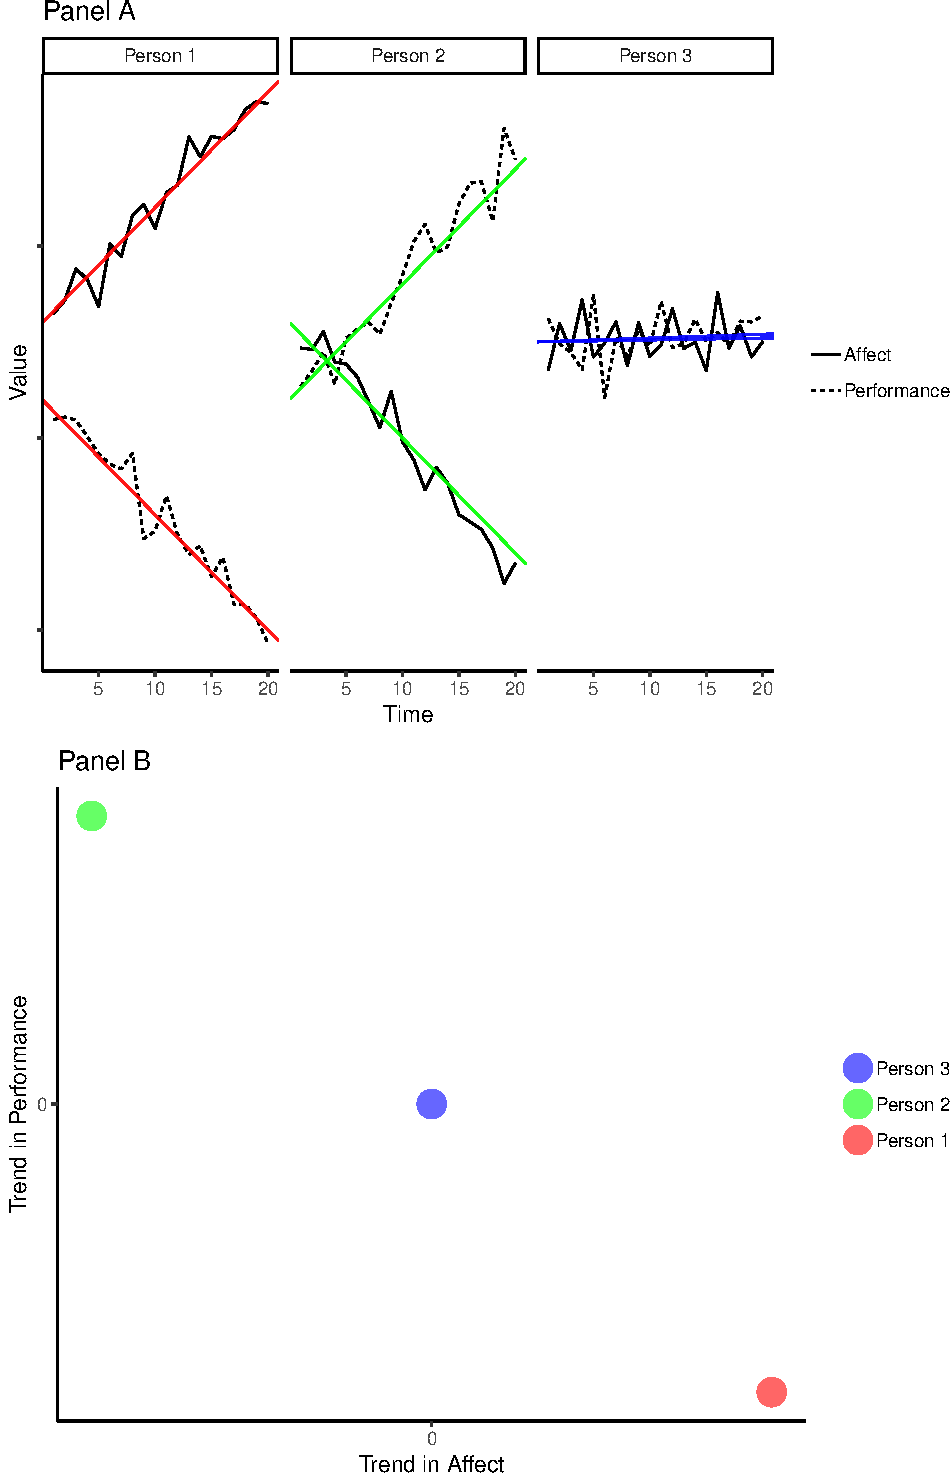
\includegraphics{figures/unnamed-chunk-10-1.pdf}
\caption{\label{fig:unnamed-chunk-10}t\label{trend}}
\end{figure}

\begin{figure}
\centering
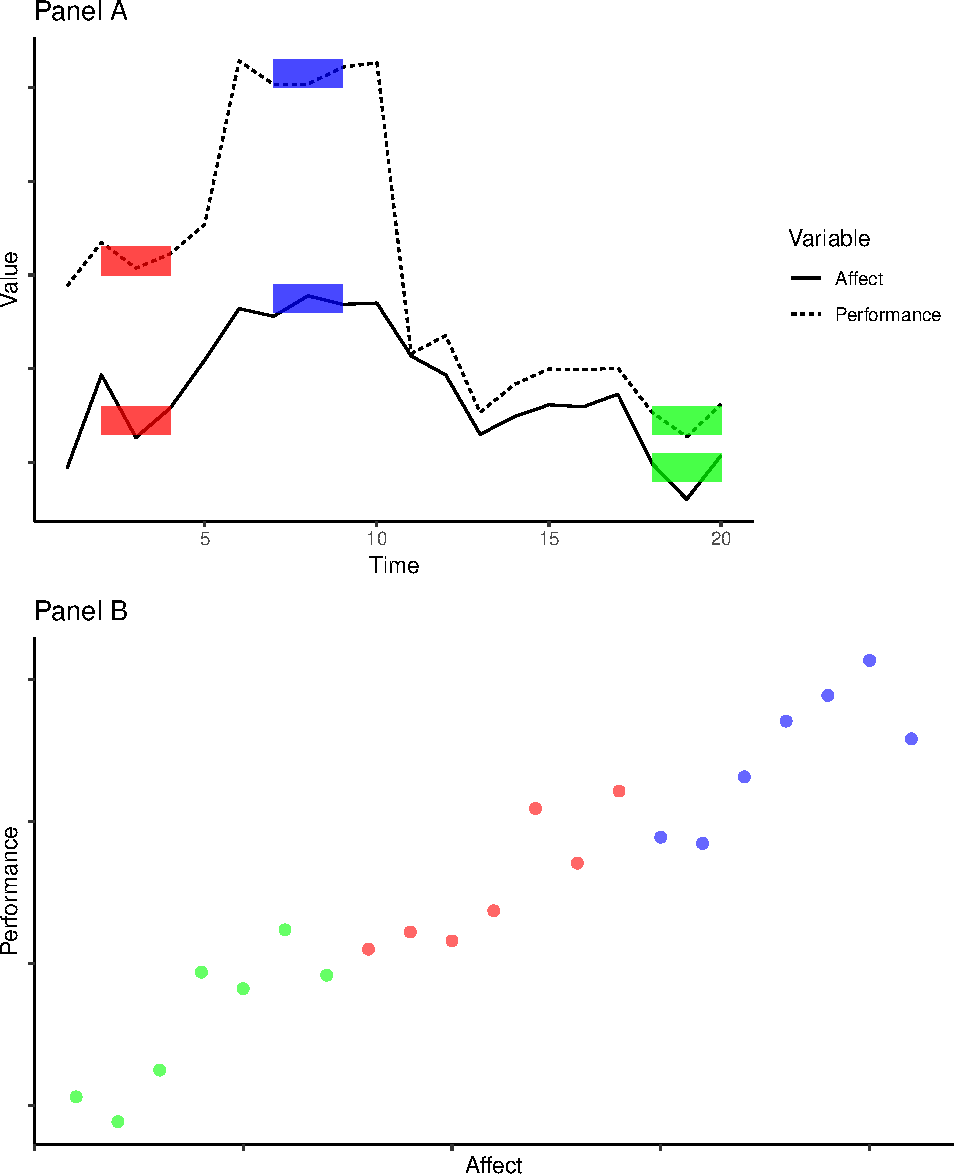
\includegraphics{figures/unnamed-chunk-11-1.pdf}
\caption{\label{fig:unnamed-chunk-11}tr\label{trend_var}}
\end{figure}

\begin{figure}
\centering
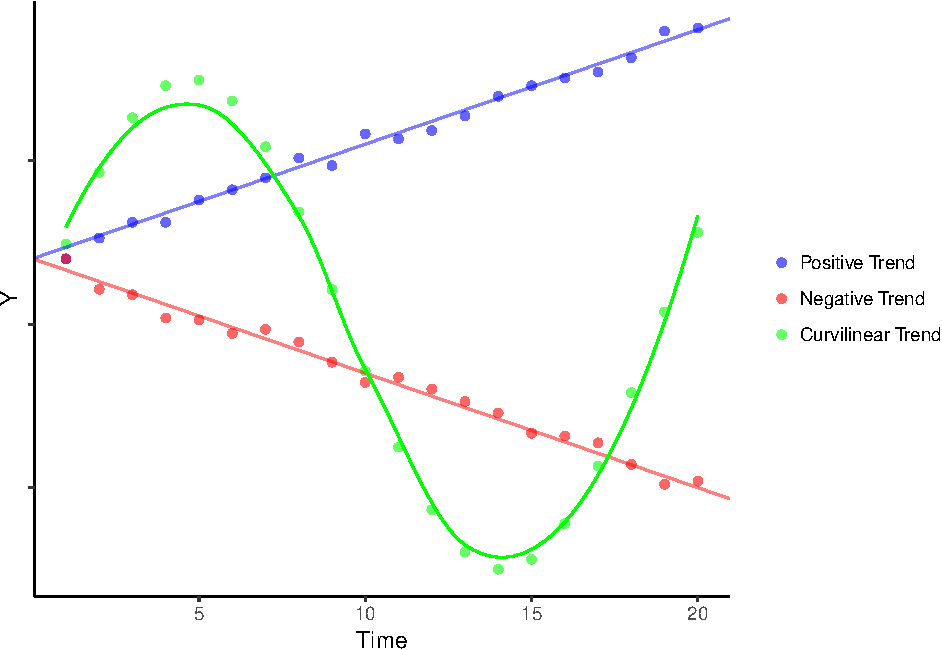
\includegraphics{figures/unnamed-chunk-12-1.pdf}
\caption{\label{fig:unnamed-chunk-12}trend to trend\label{trend_rel}}
\end{figure}

\hypertarget{models-1}{%
\subsection{Models}\label{models-1}}

Growth curves in SEM or HLM. Bivariate growth curves.

\hypertarget{dynamics}{%
\section{Dynamics}\label{dynamics}}

\hypertarget{mediation}{%
\section{Mediation}\label{mediation}}

\hypertarget{discussion}{%
\section{Discussion}\label{discussion}}

Points to include. 1) Econometrics modeling levels vs.~modeling
differences. 2) Keep in mind you might see weird stuff in the
literature. X at time 1 relates to Z at time 2, which relates to Y at
time 3, but none are measured repeatedly across time. This is no good.

\newpage

\hypertarget{references}{%
\section{References}\label{references}}

\begin{Shaded}
\begin{Highlighting}[]
\KeywordTok{r_refs}\NormalTok{(}\DataTypeTok{file =} \StringTok{"references.bib"}\NormalTok{)}
\end{Highlighting}
\end{Shaded}

\setlength{\parindent}{-0.5in}
\setlength{\leftskip}{0.5in}

\hypertarget{refs}{}
\leavevmode\hypertarget{ref-beal_esm_2015}{}%
Beal, D. J. (2015). ESM 2.0: State of the art and future potential of
experience sampling methods in organizational research. \emph{Annu. Rev.
Organ. Psychol. Organ. Behav.}, \emph{2}(1), 383--407.

\leavevmode\hypertarget{ref-hardy_interrelationships_2018}{}%
Hardy, J. H., Day, E. A., \& Steele, L. M. (2018). Interrelationships
Among Self-Regulated Learning Processes: Toward a Dynamic Process-Based
Model of Self-Regulated Learning. \emph{Journal of Management},
0149206318780440.
doi:\href{https://doi.org/10.1177/0149206318780440}{10.1177/0149206318780440}

\leavevmode\hypertarget{ref-ilgen_computational_2000}{}%
Ilgen, D. R., \& Hulin, C. L. (2000). \emph{Computational modeling of
behavior in organizations: The third scientific discipline.} American
Psychological Association.

\leavevmode\hypertarget{ref-johnson_good_2014}{}%
Johnson, R. E., Lanaj, K., \& Barnes, C. M. (2014). The good and bad of
being fair: Effects of procedural and interpersonal justice behaviors on
regulatory resources. \emph{Journal of Applied Psychology},
\emph{99}(4), 635.

\leavevmode\hypertarget{ref-jones_baby_2016}{}%
Jones, K. P., King, E. B., Gilrane, V. L., McCausland, T. C., Cortina,
J. M., \& Grimm, K. J. (2016). The baby bump: Managing a dynamic stigma
over time. \emph{Journal of Management}, \emph{42}(6), 1530--1556.

\leavevmode\hypertarget{ref-koopman_integrating_2016}{}%
Koopman, J., Lanaj, K., \& Scott, B. A. (2016). Integrating the Bright
and Dark Sides of OCB: A Daily Investigation of the Benefits and Costs
of Helping Others. \emph{Academy of Management Journal}, \emph{59}(2),
414--435.
doi:\href{https://doi.org/10.5465/amj.2014.0262}{10.5465/amj.2014.0262}

\leavevmode\hypertarget{ref-kozlowski_work_2003}{}%
Kozlowski, S. W., \& Bell, B. S. (2003). Work groups and teams in
organizations. \emph{Handbook of Psychology}, 333--375.

\leavevmode\hypertarget{ref-meier_reciprocal_2013}{}%
Meier, L. L., \& Spector, P. E. (2013). Reciprocal effects of work
stressors and counterproductive work behavior: A five-wave longitudinal
study. \emph{Journal of Applied Psychology}, \emph{98}(3), 529.

\leavevmode\hypertarget{ref-pitariu_explaining_2010}{}%
Pitariu, A. H., \& Ployhart, R. E. (2010). Explaining change: Theorizing
and testing dynamic mediated longitudinal relationships. \emph{Journal
of Management}, \emph{36}(2), 405--429.

\leavevmode\hypertarget{ref-ployhart_longitudinal_2010}{}%
Ployhart, R. E., \& Vandenberg, R. J. (2010). Longitudinal research: The
theory, design, and analysis of change. \emph{Journal of Management},
\emph{36}(1), 94--120.

\leavevmode\hypertarget{ref-ritter_understanding_2016}{}%
Ritter, K.-J., Matthews, R. A., Ford, M. T., \& Henderson, A. A. (2016).
Understanding role stressors and job satisfaction over time using
adaptation theory. \emph{Journal of Applied Psychology}, \emph{101}(12),
1655.

\leavevmode\hypertarget{ref-rosen_who_2016}{}%
Rosen, C. C., Koopman, J., Gabriel, A. S., \& Johnson, R. E. (2016). Who
strikes back? A daily investigation of when and why incivility begets
incivility. \emph{Journal of Applied Psychology}, \emph{101}(11), 1620.


\end{document}
